\section{Experiments}
\label{sec:exp}


\begin{table*}[t]
    % \footnotesize
    \centering
    \caption{\textbf{Main comparison results on LoCoMo, LongMemEval, and ALFWorld.}}
    \label{tab:exp_main}

    \begin{tabular}{>{\centering\arraybackslash}m{0.9cm} l cc cc c | cc cc c}
        \toprule
        \multirow{3}{*}{\textbf{Model}} &
        \multirow{3}{*}{\textbf{Methods}} &
        \multicolumn{5}{c}{\textbf{Conversational Benchmarks}} &
        \multicolumn{5}{c}{\textbf{Embodied Interactive Tasks}} \\
        \cmidrule(lr){3-7} \cmidrule(lr){8-12}
        & &
        \multicolumn{2}{c}{\textbf{LoCoMo}} &
        \multicolumn{2}{c}{\textbf{$^\blacktriangle$LongMemEval}} &
        \multicolumn{1}{c}{\textbf{Avg.}} &
        \multicolumn{2}{c}{\textbf{ALF-Seen$^\dagger$}} &
        \multicolumn{2}{c}{\textbf{ALF-Unseen$^\dagger$}} &
        \multicolumn{1}{c}{\textbf{Avg.}} \\
        \cmidrule(lr){3-4} \cmidrule(lr){5-6} \cmidrule(lr){7-7}
        \cmidrule(lr){8-9} \cmidrule(lr){10-11} \cmidrule(lr){12-12}
        & &
        \textbf{F1} & \textbf{L-J} &
        \textbf{F1} & \textbf{L-J} &
        \textbf{L-J} &
        \textbf{SR} & \textbf{\#Stps$\downarrow$} &
        \textbf{SR} & \textbf{\#Stps$\downarrow$} &
        \textbf{SR} \\
        \midrule



        % ===================== Base model block 1 =====================
        \multirow{9}{*}{\rotatebox[origin=c]{90}{\shortstack{\textbf{LLaMA3.3}\\\textbf{70B-Instruct}}}} &
        No-Memory         & - & - & - & - & - & 62.14 & 26.10 & 73.88 & 21.36 & 68.01 \\
        & CoN       & 30.86 & 41.72 & 30.78 & 56.44 & 49.08 & 75.00 & 19.15 & 80.60 & 17.38 & 77.80 \\
        & ReadAgent  & 28.63 & 38.25 & 24.48 & 42.62 & 40.44 & 62.86 & 26.14 & 71.64 & 22.88 & 67.25 \\
        & MemoryBank & 36.80 & 44.43 & 30.56 & 41.96 & 43.20 & 60.71 & 28.23 & 66.42 & 24.64 & 63.57 \\
        & A-MEM      & 39.39 & 49.71 & 25.83 & 38.04 & 43.88 & 62.86 & 27.53 & 70.15 & 23.79 & 66.51 \\
        & Mem0       & 25.48 & 34.58 & 30.25 & 46.81 & 40.70 & 74.29 & 19.77 & 81.34 & 17.15 & 77.82 \\
        & LangMem    & 30.91 & 35.82 & 18.36 & 24.35 & 30.09 & 72.86 & 21.25 & 79.85 & 18.30 & 76.36 \\
        & MemoryOS   & 41.39 & 48.64 & 17.59 & 39.83 & 44.24 & 57.86 & 27.94 & 65.67 & 24.46 & 61.77 \\
        & \cellcolor{hl-llama}\textbf{MemSkill} &
        \cellcolor{hl-llama}\textbf{44.21} & \cellcolor{hl-llama}\textbf{53.82} & \cellcolor{hl-llama}\textbf{31.12} & \cellcolor{hl-llama}\textbf{60.89} &
        \cellcolor{hl-llama}\textbf{57.36} &
        \cellcolor{hl-llama}\textbf{77.14} & \cellcolor{hl-llama}\textbf{18.91} &
        \cellcolor{hl-llama}\textbf{83.58} & \cellcolor{hl-llama}\textbf{16.63} &
        \cellcolor{hl-llama}\textbf{80.36} \\
        \midrule

        % ===================== Base model block 2 =====================
        \multirow{9}{*}{\rotatebox[origin=c]{90}{\shortstack{$^\blacktriangle$\textbf{Qwen3-Next}\\\textbf{80B-A3B-Instruct}}}} &
        No-Memory         & - & - & - & - & - & 63.57 & 24.61 & 60.45 & 26.57 & 62.01 \\
        & CoN       & 38.46 & 50.96 & \textbf{29.19} & 44.06 & 47.51 & 77.14 & 17.59 & 70.90 & 20.74 & 74.02 \\
        & ReadAgent  & 25.89 & 34.26 & 24.13 & 42.25 & 38.26 & 73.57 & 20.21 & 65.67 & 23.28 & 69.62 \\
        & MemoryBank & 29.56 & 44.15 & 8.45 & 26.37 & 35.26 & 63.57 & 23.68 & 52.24 & 29.01 & 57.91 \\
        & A-MEM      & 36.43 & 50.30 & 13.84 & 36.59 & 43.45 & 55.71 & 27.42 & 54.48 & 28.60 & 55.10 \\
        & Mem0       & 23.29 & 33.68 & 27.36 & 46.20 & 39.94 & 71.43 & 19.89 & 64.93 & 23.32 & 68.18 \\
        & LangMem    & 28.17 & 32.94 & 18.35 & 23.86 & 28.40 & 73.57 & 19.76 & 64.18 & 23.58 & 68.88 \\
        & MemoryOS   & 39.86 & 47.37 & 15.97 & 39.25 & 43.31 & 62.14 & 25.64 & 50.75 & 30.35 & 56.45 \\
        & \cellcolor{hl-qwen}\textbf{MemSkill} &
        \cellcolor{hl-qwen}\textbf{42.08} & \cellcolor{hl-qwen}\textbf{54.14} & \cellcolor{hl-qwen}25.29 & \cellcolor{hl-qwen}\textbf{60.40} &
        \cellcolor{hl-qwen}\textbf{57.27} &
        \cellcolor{hl-qwen}\textbf{85.71} & \cellcolor{hl-qwen}\textbf{13.84} &
        \cellcolor{hl-qwen}\textbf{76.87} & \cellcolor{hl-qwen}\textbf{18.16} &
        \cellcolor{hl-qwen}\textbf{81.29} \\
        \bottomrule

        \multicolumn{12}{l}{\small \textbf{Bold} indicates the best score within each base model block; $^\blacktriangle$ indicates transfer evaluation only.} \\
        \multicolumn{12}{l}{\small $^\dagger$ indicates evaluation with in-context demonstrations. Appendix~\ref{appendix:more_exp} reports more baselines and datasets.} \\
        \\
    \end{tabular}
\end{table*}



\subsection{Experiment Setup}
\label{sec:exp_setup}



\textbf{Datasets and Baselines.}
We evaluate MemSkill on four benchmarks: LoCoMo~\citep{maharana2024evaluating-locomo}, LongMemEval~\citep{wu2024longmemeval}, HotpotQA~\cite{yang2018hotpotqa}, and ALFWorld~\cite{shridhar2020alfworld}, where HotpotQA is used in Section~\ref{sec:exp_shift} to study skill transfer under distribution shift. The remaining three benchmarks cover two representative settings. 
(i) \textit{Conversational Benchmarks} include LoCoMo and LongMemEval, which evaluate memory construction from long, dialogue-style interaction histories. 
For these datasets, we report F1-score (F1) and an LLM-based judge score (L-J).
(ii) \textit{Embodied Interactive Tasks} are evaluated on ALFWorld with two standard subsets, ALF-Seen and ALF-Unseen, and we report success rate (SR) and the number of environment interaction steps (\#Stps).
Appendix~\ref{appendix:exp_eval} provides dataset splits.



We compare MemSkill against several strong baselines: (1) \textbf{No-Memory}, which answers directly without an external memory; (2) \textbf{CoN}~\citep{yu2024chain}; (3) \textbf{ReadAgent}~\citep{lee2024human}; (4) \textbf{MemoryBank}~\citep{zhong2024memorybank}; (5) \textbf{A-MEM}~\citep{xu2025mem}; (6) \textbf{Mem0}~\citep{chhikara2025mem0}; (7) \textbf{LangMem}~\citep{LangMem}; and (8) \textbf{MemoryOS}~\citep{kang2025memory}.
Overall, this setup spans diverse benchmarks and baselines, enabling a broad and consistent comparison across diverse settings.






\textbf{Implementation Details.}
We instantiate $f_{\theta}^{\mathrm{ctx}}$, $f_{\theta}^{\mathrm{skill}}$, and $f_{\theta}^{\mathrm{score}}$ as independent lightweight multilayer perceptrons (MLPs), and use LLaMA-3.3-70B-Instruct~\citep{grattafiori2024llama} and Qwen3-Next-80B-A3B-Instruct~\citep{yang2025qwen3} as the base LLMs, accessed through an API service. Unless otherwise specified, we train MemSkill on LLaMA and use Qwen only for transfer experiments. LongMemEval is also evaluated in a transfer setting, where we directly apply the skills learned on LoCoMo without further training.


During training, we optimize the controller with PPO~\cite{schulman2017proximal}. MemSkill constructs memory at the span level; on conversational benchmarks, each dialogue session is a processing unit, and the controller selects $K{=}3$ skills per unit. We instantiate $e(\cdot)$ with Qwen3-Embedding-0.6B~\citep{yang2025qwen3}, also used as the memory retriever, and retrieve up to 20 memory items for MemSkill and all baselines for consistency. For the designer, skill evolution is triggered every 100 training steps, with at most 3 skill edits per evolution round. For ALFWorld, we cap environment interactions at 50 steps.


At evaluation time, we keep the same span-level formulation and set the span/chunk size to 512 by default, while keeping the overall procedure unchanged. Unless otherwise specified, we use $K{=}7$ skills for LoCoMo and LongMemEval at evaluation time, and $K{=}5$ for ALFWorld. Additional implementation details and prompt templates are provided in Appendix~\ref{appendix:imple_detail} and Appendix~\ref{appendix:prompts}.






\begin{figure*}[t]
	\centering
	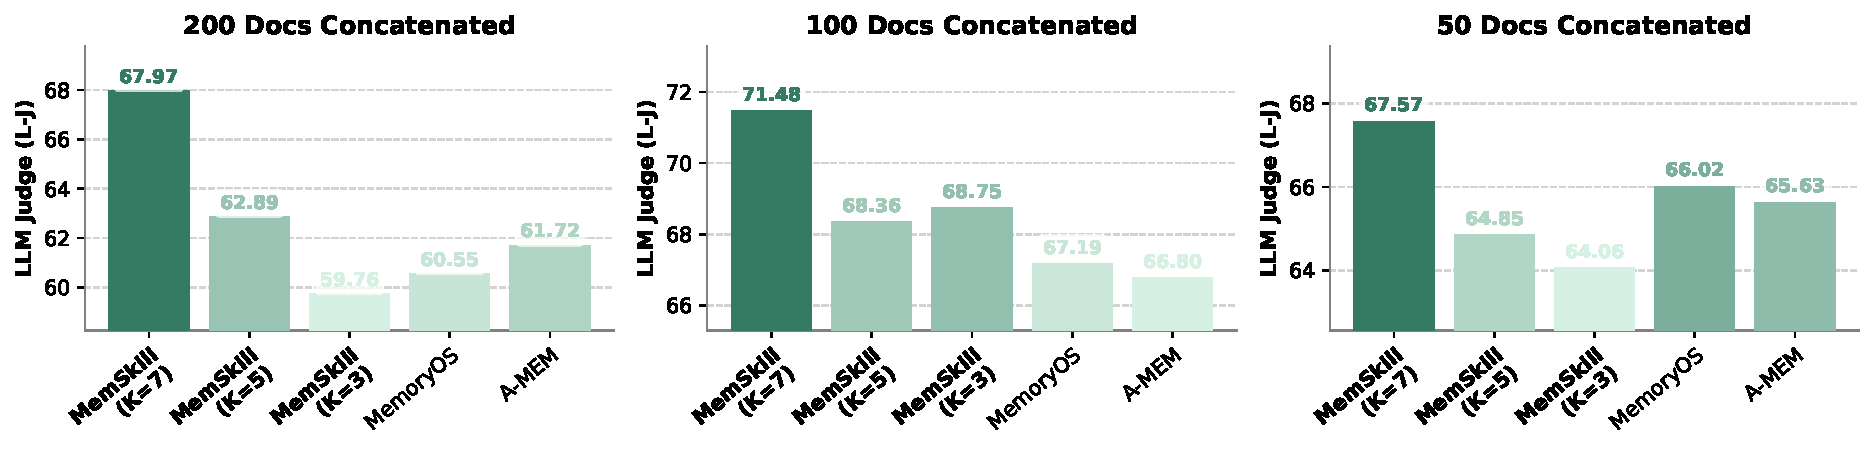
\includegraphics[width=1.0\linewidth]{figs/hotpotqa_transfer_bars.pdf}
        \caption{\textbf{Skill generalization under distribution shift on HotpotQA.} We transfer the LoCoMo-trained skill bank to HotpotQA and evaluate three context-length settings (50/100/200 concatenated documents) following~\citep{yu2025memagent}. Bars show LLM-judge (L-J) under LLaMA with different Top-$K$ skill counts, compared to MemoryOS and A-MEM.}
	\label{fig:hotpot_shift}
\end{figure*}





\subsection{Comparison Experiments}
\label{sec:exp_main}



\textbf{Effectiveness across conversational and embodied settings.}
Table~\ref{tab:exp_main} summarizes the main comparison results on LoCoMo, LongMemEval, and ALFWorld. Across these datasets, MemSkill achieves the strongest overall performance among all compared methods. On conversational benchmarks, MemSkill attains the best LLM-judge scores on both LoCoMo and LongMemEval within each base-model block, indicating higher-quality constructed memories. 
In comparison, prior methods such as MemoryBank, A-MEM, and MemoryOS use fixed, manually specified memory procedures for extraction and revision, whereas MemSkill learns and evolves its skills from interaction, enabling better adaptation across contexts.
On ALFWorld, MemSkill achieves the highest success rates on both seen and unseen splits, indicating that skill-guided memory construction can benefit interactive decision making, whereas other baselines are less reliable at leveraging memory to support long-horizon action execution.
Overall, the results show that MemSkill is effective across diverse settings.





\textbf{Generalization across base models.}
A key advantage of MemSkill is strong generalization across base models. We train MemSkill only with LLaMA and directly transfer the learned skills to Qwen without retraining. Despite this strict transfer setting, MemSkill remains competitive and outperforms strong baselines on both conversational and embodied evaluations, showing that the evolved skills capture reusable memory behaviors that can be instantiated by different underlying LLMs.


\textbf{Cross-dataset transfer.}
MemSkill also generalizes across datasets within the same broad setting. In particular, LongMemEval is evaluated purely by transferring the skill bank learned on LoCoMo, yet MemSkill achieves the best results among all methods, suggesting that the learned skills are not overfit to a single benchmark. Section~\ref{sec:exp_shift} studies transfer under more pronounced distribution shifts.










\subsection{Skill Generalization Under Distribution Shift}
\label{sec:exp_shift}



Beyond transfer within dialogue-style memory benchmarks, we evaluate whether learned skills generalize under a distribution shift in interaction format and evidence structure. 
Concretely, we directly apply the skill bank trained on LoCoMo to HotpotQA, where inputs are long-form, document-style narratives rather than multi-turn dialogues. 
Following the protocol in~\citep{yu2025memagent}, we test three context-length settings with increasing difficulty, corresponding to different numbers of concatenated documents (i.e., 50/100/200). 
All results in this section use LLaMA as the base model and report the LLM-judge score (L-J). 
For baselines, we include MemoryOS and A-MEM, the most competitive methods on conversational benchmarks in Table~\ref{tab:exp_main}, and omit weaker alternatives for clarity.



Figure~\ref{fig:hotpot_shift} shows that MemSkill transfers strongly to HotpotQA across all three context sizes. 
MemSkill consistently outperforms strong baselines such as MemoryOS and A-MEM, with gains becoming more pronounced in the challenging long-context setting.
These results suggest that the learned memory skills are not tied to dialogue-specific surface forms, but capture reusable extraction and revision behaviors that remain effective as input structure and retrieval demands change.



The same plots also reveal mild sensitivity to the number of selected skills $K$. Increasing $K$ generally improves performance, with $K{=}7$ achieving the best results across all three settings, while smaller $K$ can under-utilize the skill bank under longer contexts. Overall, the trend indicates that MemSkill benefits from composing multiple skills when the context becomes longer and noisier, while still maintaining strong transfer without any HotpotQA-specific training.



\begin{figure*}[t]
	\centering
	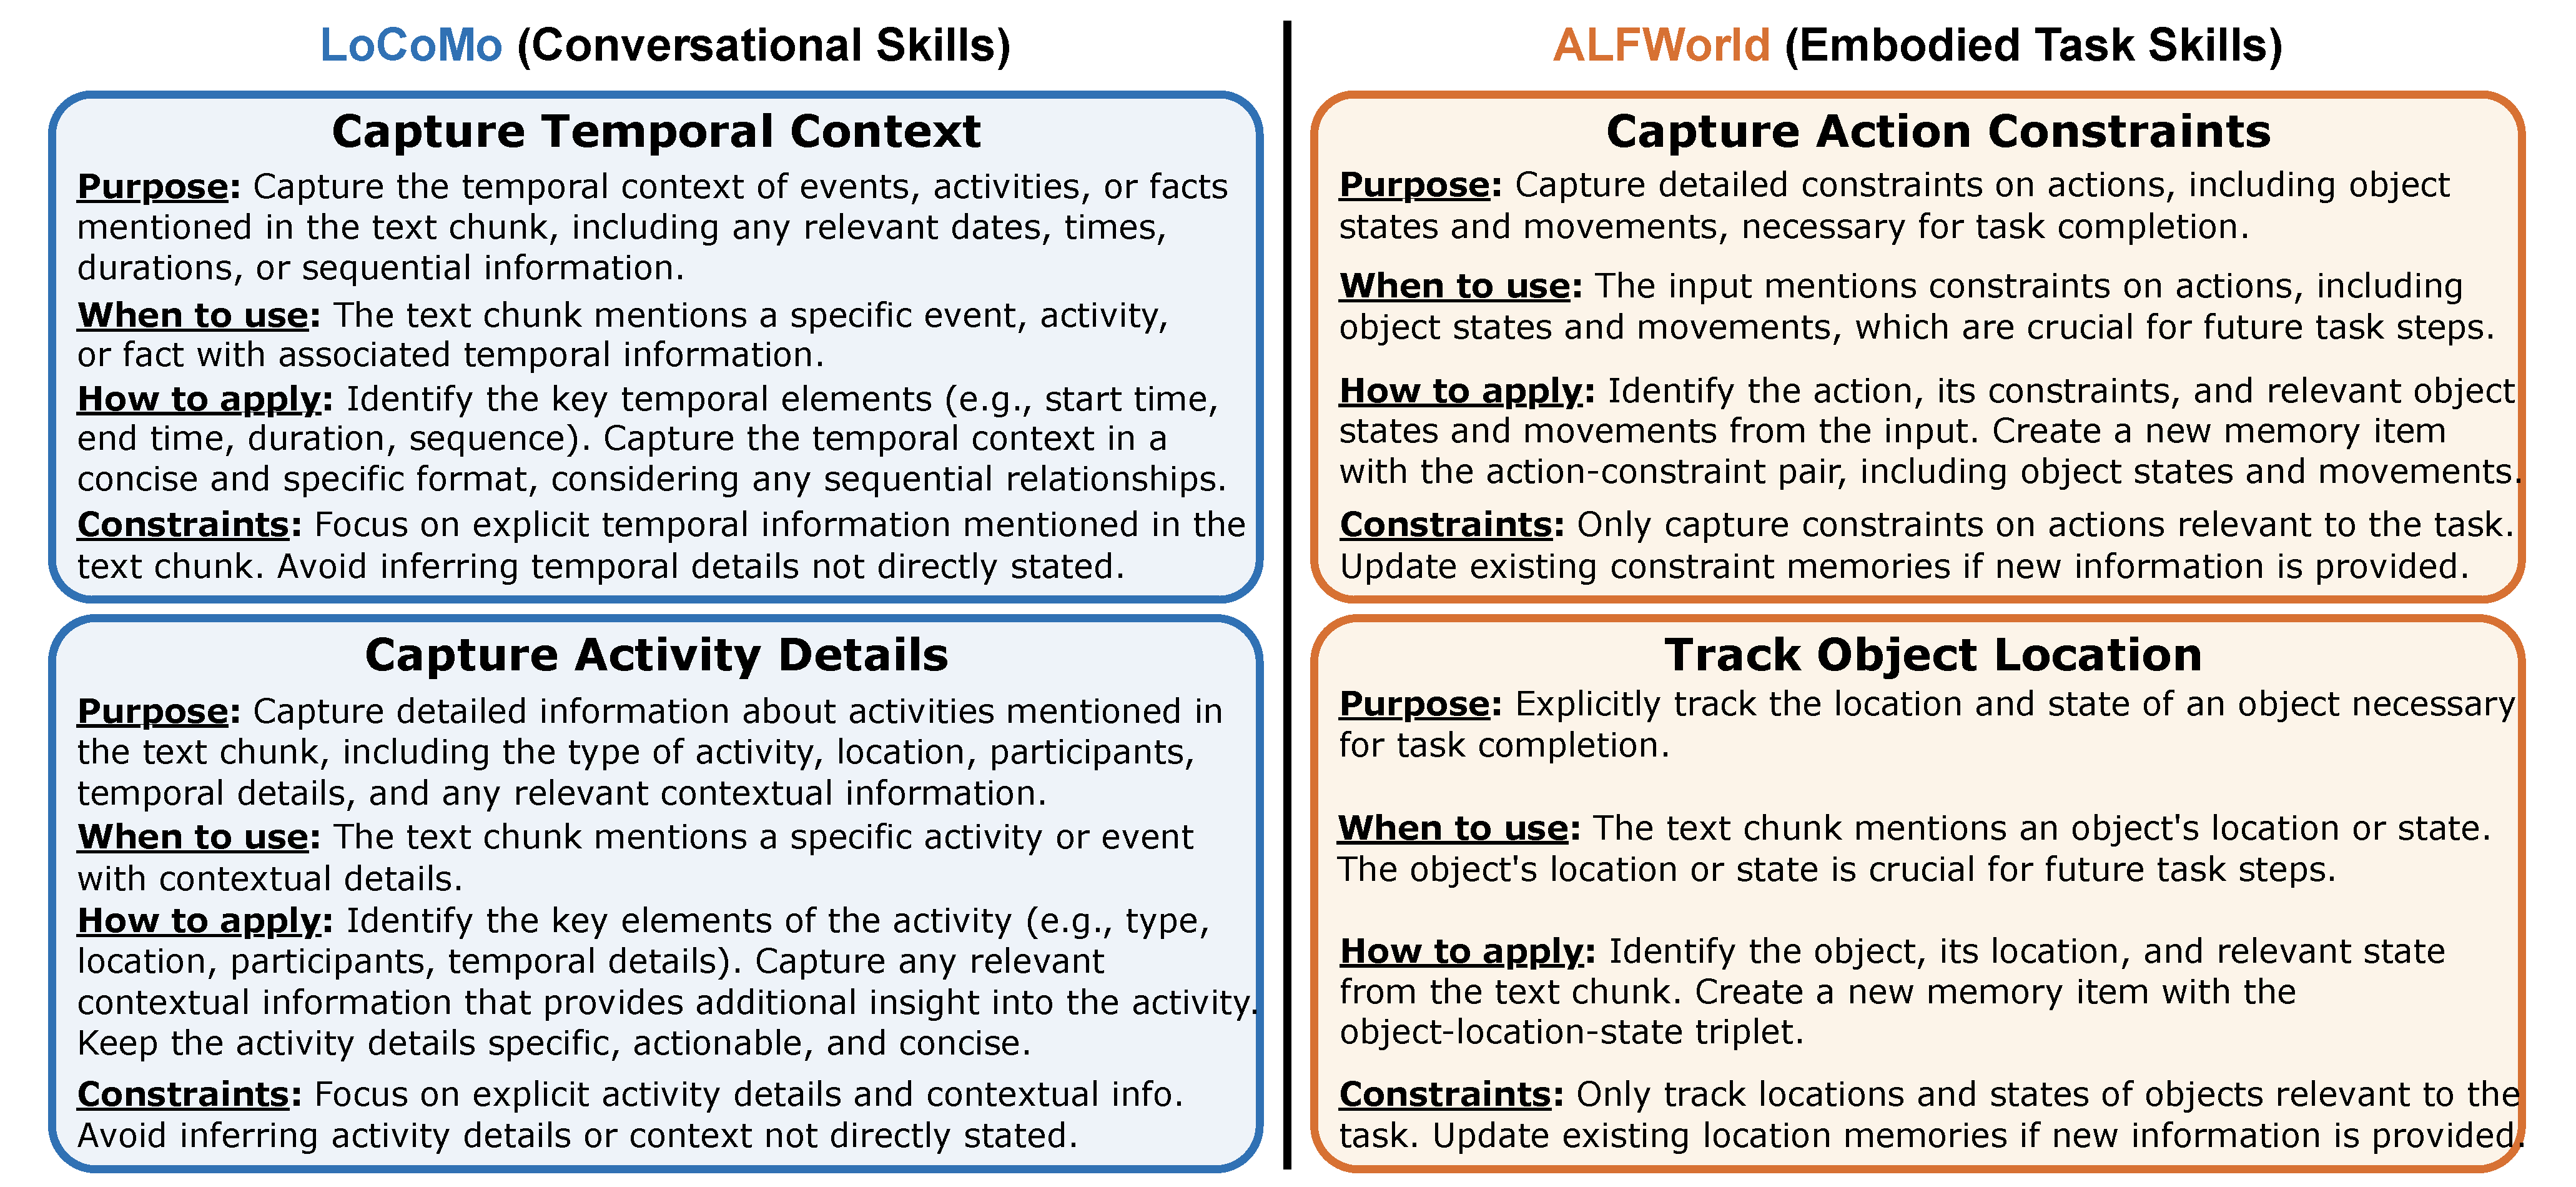
\includegraphics[width=1.0\linewidth]{figs/case_study.pdf}
        \caption{\textbf{Case study.} We show representative evolved skills learned on LoCoMo and ALFWorld.}
	\label{fig:case_study}
\end{figure*}




\subsection{Ablation Study}\label{sec:ablation}


We perform ablations to disentangle the contributions of (i) learning to select skills and (ii) evolving the skill bank. Table~\ref{tab:ablation_locomo} reports LLM Judge (L-J) results on LoCoMo under both base models (LLaMA and Qwen). 
As shown, \textbf{w/o controller (w/o Ctrl)} replaces the learned controller with random skill selection while keeping the rest of the pipeline unchanged. 
\textbf{w/o designer (w/o Des)} disables the designer and fixes the skill bank to the four initial primitives. 
\textbf{Refine-only (Ref.-only)} allows the designer to refine existing skills but prohibits adding new ones.



Across both base models, removing either component consistently degrades performance, confirming that MemSkill benefits from both targeted skill selection and skill evolution. 
In particular, random skill selection leads to a clear drop from the default setting, highlighting the importance of learning to choose relevant skills rather than providing arbitrary ones. 
Disabling the designer yields an even larger degradation, especially under Qwen, suggesting that evolving the skill bank is important for learning reusable memory behaviors that generalize beyond a fixed, manually specified operation set. 
Finally, refinement-only consistently outperforms static skills on both LLaMA and Qwen, with a particularly large gain under Qwen, yet remains below the default setting, indicating that introducing new skills yields additional benefits beyond refining the initial primitives.


\begin{table}[h]
    % \footnotesize
    \centering
    \caption{\textbf{LoCoMo ablation} (L-J).}
    \label{tab:ablation_locomo}
    \begin{tabular}{lcc}
        \toprule
        \textbf{Variant} & \textbf{LLaMA} & \textbf{Qwen} \\
        \midrule
        \textbf{MemSkill} & \textbf{53.82} & \textbf{54.14} \\
        \quad w/o Ctrl & 48.43 & 42.84 \\
        \quad w/o Des & 46.50 & 36.15 \\
        \quad Ref.-only & 47.45 & 48.88 \\
        \bottomrule
    \end{tabular}
\end{table}








\subsection{Discussion}
\label{sec:case_study}




\textbf{Case study.}
To make MemSkill more interpretable, we inspect the final evolved skill bank and report representative skills from LoCoMo and ALFWorld. 
As shown in Figure~\ref{fig:case_study}, the learned skills show clear domain specialization. 
LoCoMo skills emphasize temporal context and activity details, suggesting that dialogue memory benefits from lightweight event structure. In contrast, ALFWorld skills focus on action constraints and object locations, showing that embodied tasks require actionable world-state memories for multi-step execution.
Overall, the evolved skill bank reflects recurring information needs from the data, rather than a fixed notion of what to remember.

Together, these skills show that MemSkill distills and refines reusable memory behaviors from interaction data, reducing reliance on hand-crafted memory designs. Appendix~\ref{appendix:case_study} gives more examples.






\textbf{Cost analysis.}
We conduct a runtime cost analysis on LoCoMo using LLaMA, additionally including \textbf{LightMem}~\citep{fang2025lightmem} as a baseline. We report L-J, input/output tokens, and LLM calls, accounting for all inference-time LLM calls from memory extraction and query answering, excluding LLM-judge calls used only for evaluation. Since MemSkill learns and evolves the skill bank before deployment, this preparation cost is amortized over repeated use, with further evolution triggered only occasionally. We therefore focus on runtime cost as the practical efficiency measure. At inference time, MemSkill constructs memory at the span level rather than turn by turn, substantially reducing LLM calls. To show this trade-off, we vary the span size (SS) and report the quality-cost frontier in Table~\ref{tab:cost_analysis_chunk}.








MemSkill achieves a stronger quality-cost trade-off than prior baselines. With moderate span sizes, it obtains higher L-J scores while using fewer input/output tokens and LLM calls. In particular, Span Size=512 offers the best overall balance, achieving the highest quality with much lower runtime cost than MemoryOS, A-MEM, and LightMem. This suggests span-level construction reduces redundant LLM calls without sacrificing memory quality. Larger span sizes reduce cost, but may hurt performance because each memory update covers a longer span. This makes span size a knob for adapting MemSkill to different efficiency requirements.




\begin{table}[h]
    \footnotesize
    \centering
    \caption{\textbf{Cost analysis on LoCoMo.}}
    \label{tab:cost_analysis_chunk}
    \begin{tabular}{lcccc}
        \toprule
        \textbf{Setting} & \textbf{L-J} & \textbf{In (K)} & \textbf{Out (K)} & \textbf{Calls} \\
        \midrule
        MemoryOS  & 48.64 & 1013 & 165 & 1288 \\
        A-MEM     & 49.71 & 2850 & 362 & 1548 \\
        LightMem  & 51.95 & 789  & 209 & 685  \\
        \midrule
        \cellcolor{hl-llama}\textbf{Ours} (SS=128)  & \cellcolor{hl-llama}53.14 & \cellcolor{hl-llama}622 & \cellcolor{hl-llama}57 & \cellcolor{hl-llama}376 \\
        \cellcolor{hl-llama}\textbf{Ours} (SS=256)  & \cellcolor{hl-llama}51.61 & \cellcolor{hl-llama}390 & \cellcolor{hl-llama}19 & \cellcolor{hl-llama}270 \\
        \cellcolor{hl-llama}\textbf{Ours} (SS=512)  & \cellcolor{hl-llama}53.82 & \cellcolor{hl-llama}249 & \cellcolor{hl-llama}18 & \cellcolor{hl-llama}215 \\
        \cellcolor{hl-llama}\textbf{Ours} (SS=1024) & \cellcolor{hl-llama}48.11 & \cellcolor{hl-llama}188 & \cellcolor{hl-llama}11 & \cellcolor{hl-llama}187 \\
        \cellcolor{hl-llama}\textbf{Ours} (SS=2048) & \cellcolor{hl-llama}50.46 & \cellcolor{hl-llama}178 & \cellcolor{hl-llama}10 & \cellcolor{hl-llama}185 \\
        \bottomrule
    \end{tabular}
\end{table}
